\section{Application Interface}

When you are logged in, You are redirected to the main page that contains the
auctions currently available in the application. Click on one of it to see
details and make a bid.

As you can see from the \figref{fig:main-page}, at each top of the application
page there is a drop-down menu to be able to access all sections of the app at
any time.

\begin{figure}[htb]
	\centering
	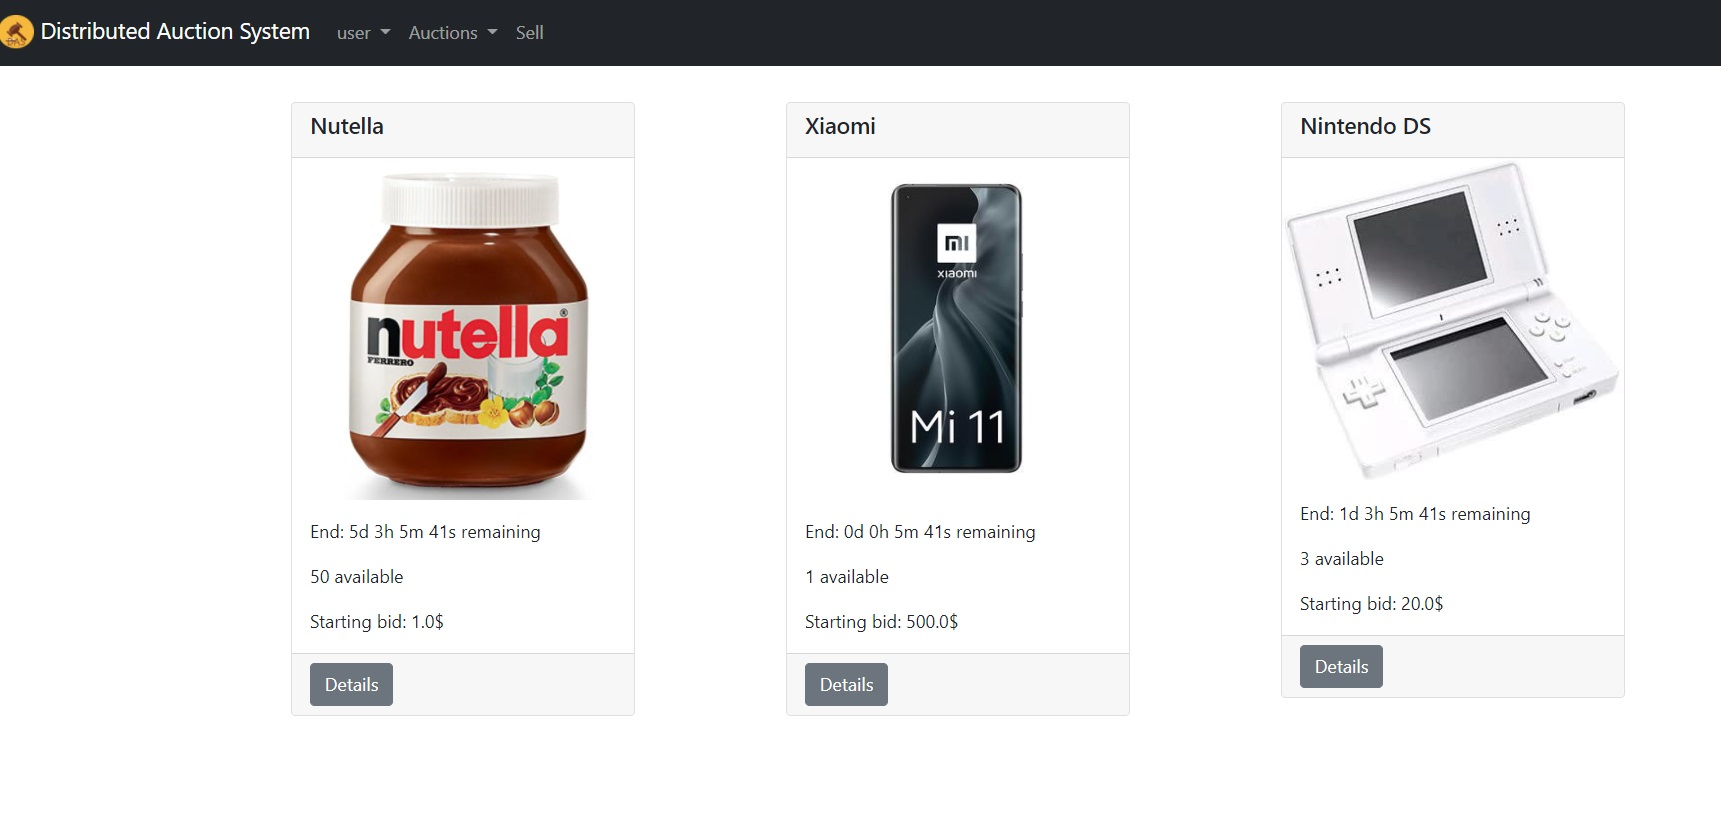
\includegraphics[width=1\textwidth]{img/main-page.jpg}
	\caption{Application main page}\label{fig:main-page}
\end{figure}

\subsection{User Section}

\subsubsection{Modify Password}

To modify your password you have to click on the User section on the top page
menu and then to press ``Modify Password''. In the page shown in
\figref{fig:modify} insert your old password and then insert twice the new
password that you desired. Then, click on the button ``Modify''. You will see a
message that says if the operation is done correctly or not. If no error occurs,
you can return to the home page clicking on the button ``Home''.

\begin{figure}[htb]
	\centering
	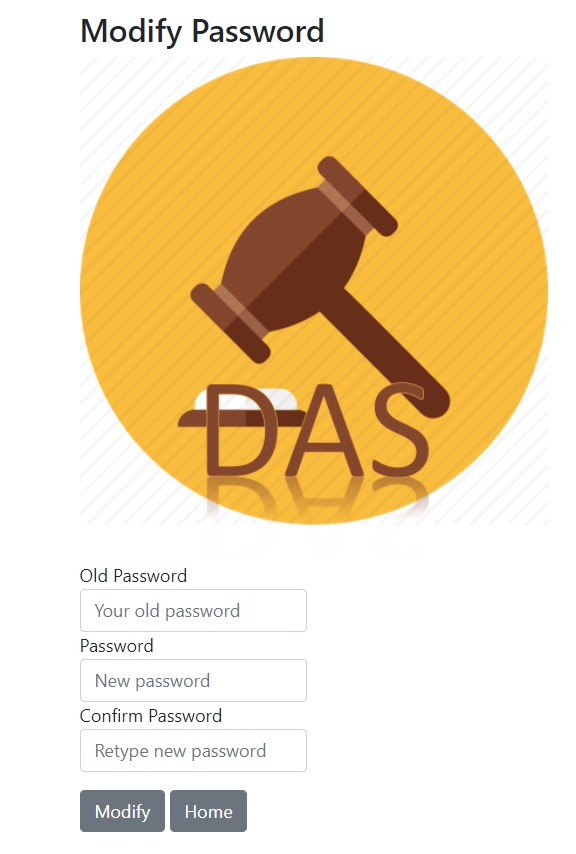
\includegraphics[width=\textwidth]{img/modify.jpg}
	\caption{Modify Password page}\label{fig:modify}
\end{figure}

\subsubsection{Logout}

To logout you have to click on the User section on the top page menu and then to
press ``Logout''. Now, if all is done correctly, you will see again the Login
page.

\subsection{Auctions Section}

%Auction List gia' descritta all'inizio

\subsubsection{MyAuctions}

The page ``MyAuctions'' has the same structure of \figref{fig:main-page} but
contains only objects that you have sold or that you want to sell.

\subsubsection{MyOffers}

Also the page ``MyOffers'' has the same structure of \figref{fig:main-page} and
contains all the objects where you have done a bid, both with finished or in
progress auctions.

\subsubsection{Select Auction}

In the pages ``Auction List'', ``MyAuctions'' and ``MyOffers'' you can click on
an auction to see its details. There are two possible detail pages:
\begin{description}
	\item[Agent detail page] If you are the owner of the selected object,
		you will see on the left your auction information, the momentary
		total gain and objects sold (they will become definitive at the
		end of auction time). On the right you can see the list of
		winning offers. All is shown in \figref{fig:detail-seller}. To
		delete the auction, you can press the button ``Delete Auction''.
	\item[Bidder detail page] If you are a customer you will see, as in
		\figref{fig:detail-customer}, the general auction information
		and the minimum bid to momentary win the quantity of objects you
		prefer.  On the right side you can bid, inserting the offer and
		the desired number of objects. Then, you have to press the
		button ``Send Bid''.  If all is done correctly, you will see if
		your offer is momentary a winning one or not, as shown in
		\figref{fig:bid}. The bid status is updated real time. If you
		see false in the column ``is winning'', this means that to win
		you have to do another bid. You can delete your bid pressing the
		button ``Delete'', on the row with the offer to cancel. At the
		end of the time, open the detail page, you will see if succeeded
		in buy the object or not, as shown in \figref{fig:win}.
\end{description}

\begin{figure}[htb]
	\centering
	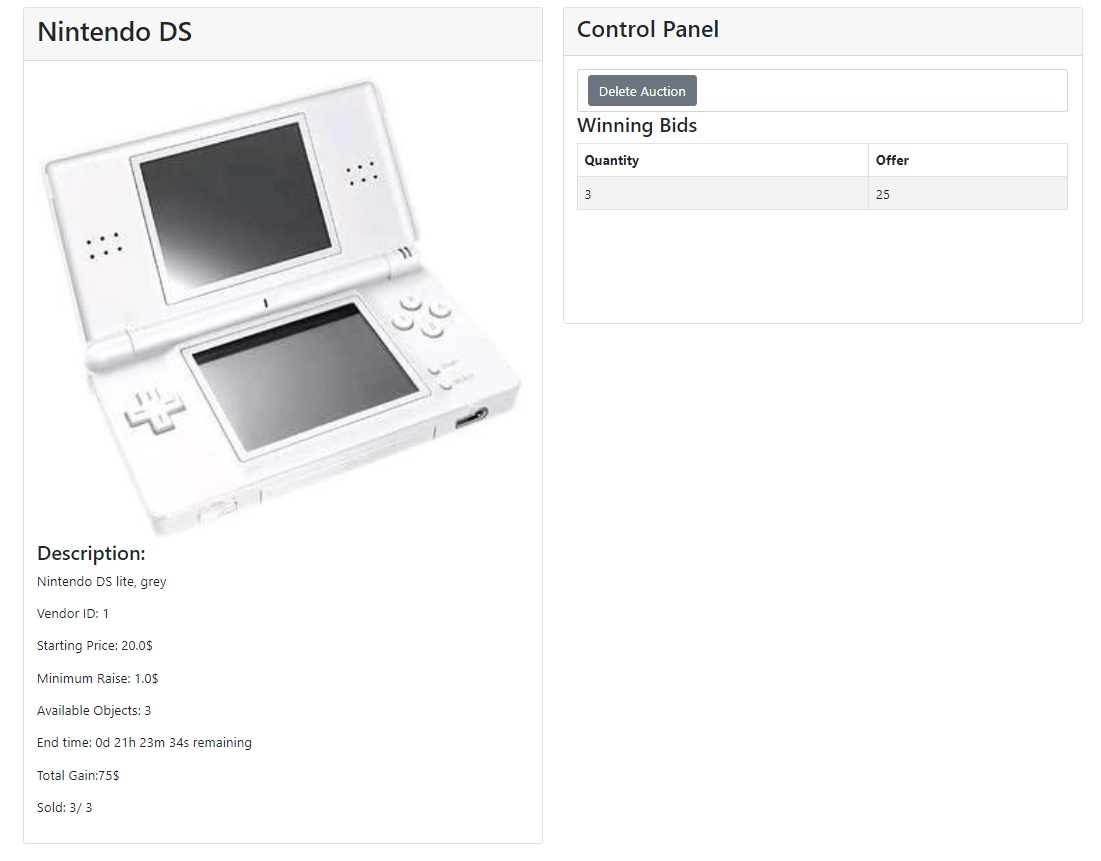
\includegraphics[width=\textwidth]{img/detail_seller.jpg}
	\caption{Details of an object from the point of view of its
	seller}\label{fig:detail-seller}
\end{figure}

\begin{figure}[htb]
	\centering
	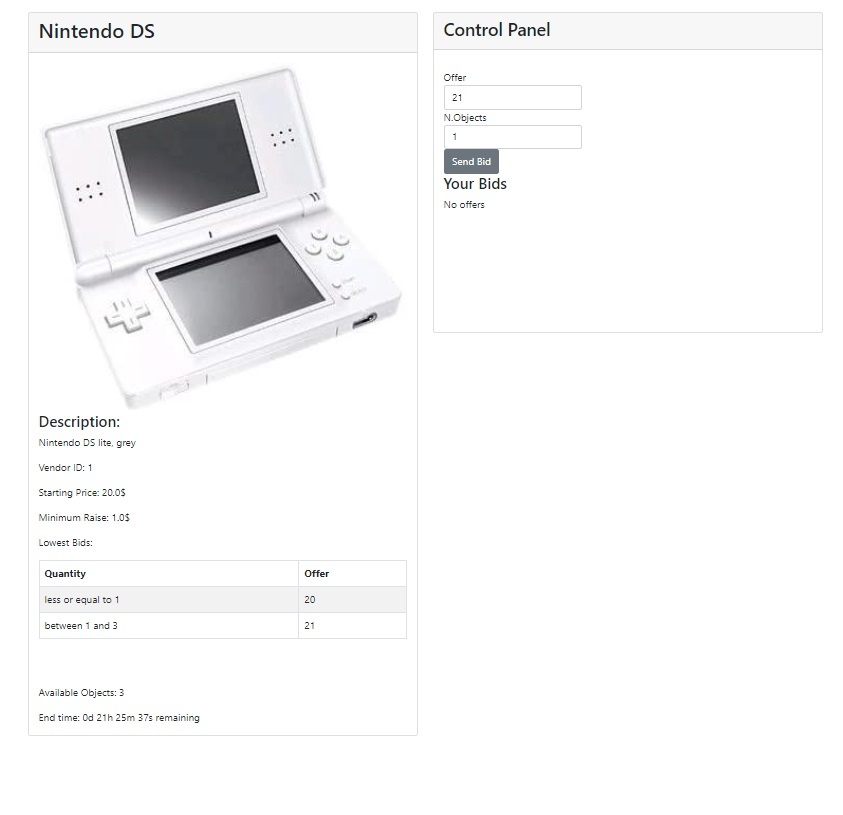
\includegraphics[width=\textwidth]{img/detail_customer.jpg}
	\caption{Details of an object from the point of view of a customer,
	without offers done}\label{fig:detail-customer}
\end{figure}

\begin{figure}[htb]
	\centering
	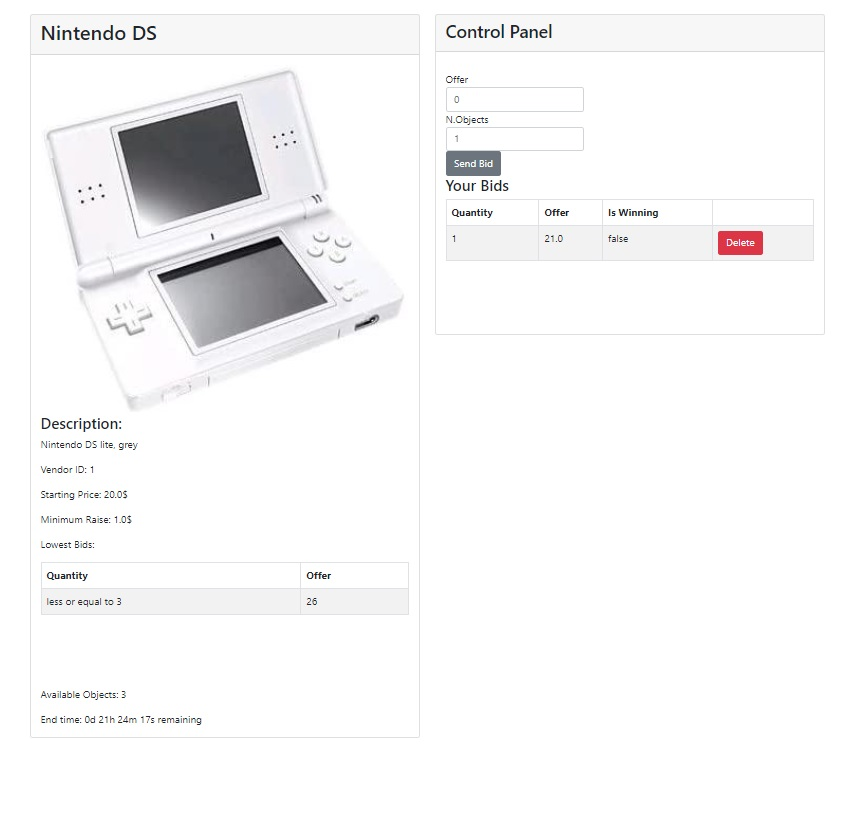
\includegraphics[width=\textwidth]{img/bid.jpg}
	\caption{Details of an object from the point of view of a customer, with
	offers done}\label{fig:bid}
\end{figure}


\begin{figure}[htb]
	\centering
	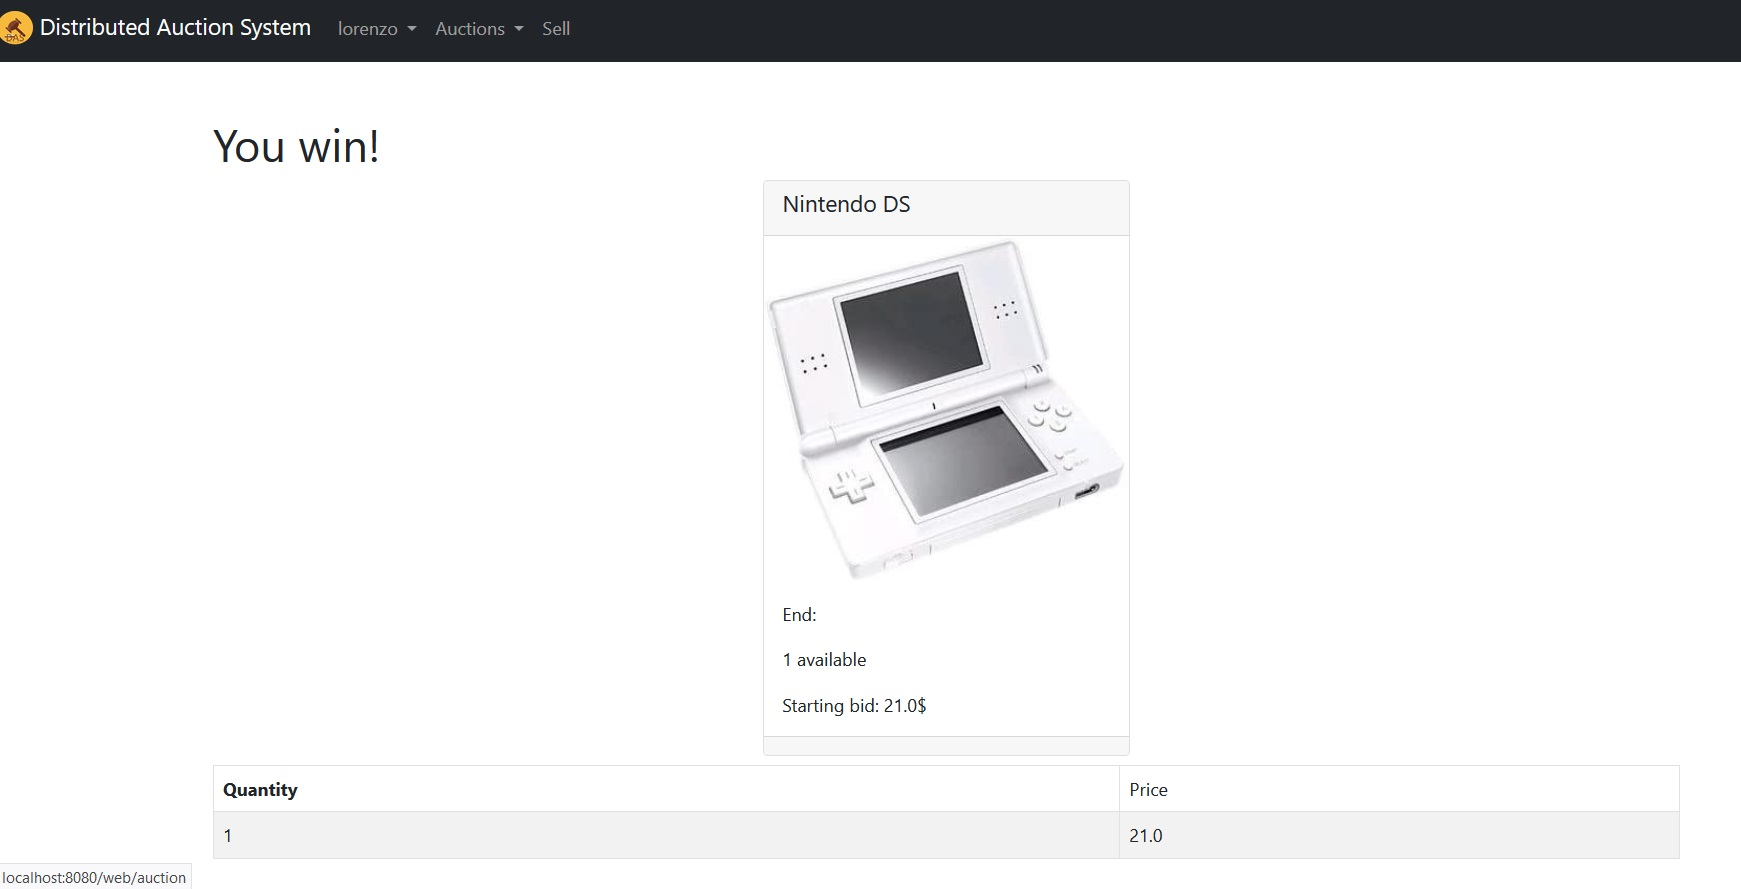
\includegraphics[width=\textwidth]{img/win.jpg}
	\caption{Page for the end of an auction on customer side}\label{fig:win}
\end{figure}


\subsection{Sell Section}

To create a new auction you have to click on the Sell section on the top page
menu. You are redirected to a page where you have to fill out a form, writing
the name of the auction, the minimum bid and the minimum raise you accept for
that auction, the number of items you want to sell for this auction, the date
and time you want the auction to end and a description of the items. It is also
necessary to upload an image of the items for sale. Then, click on the button
``Sell''. If no errors are shown, you have created a new auction.

\begin{figure}[htb]
	\centering
	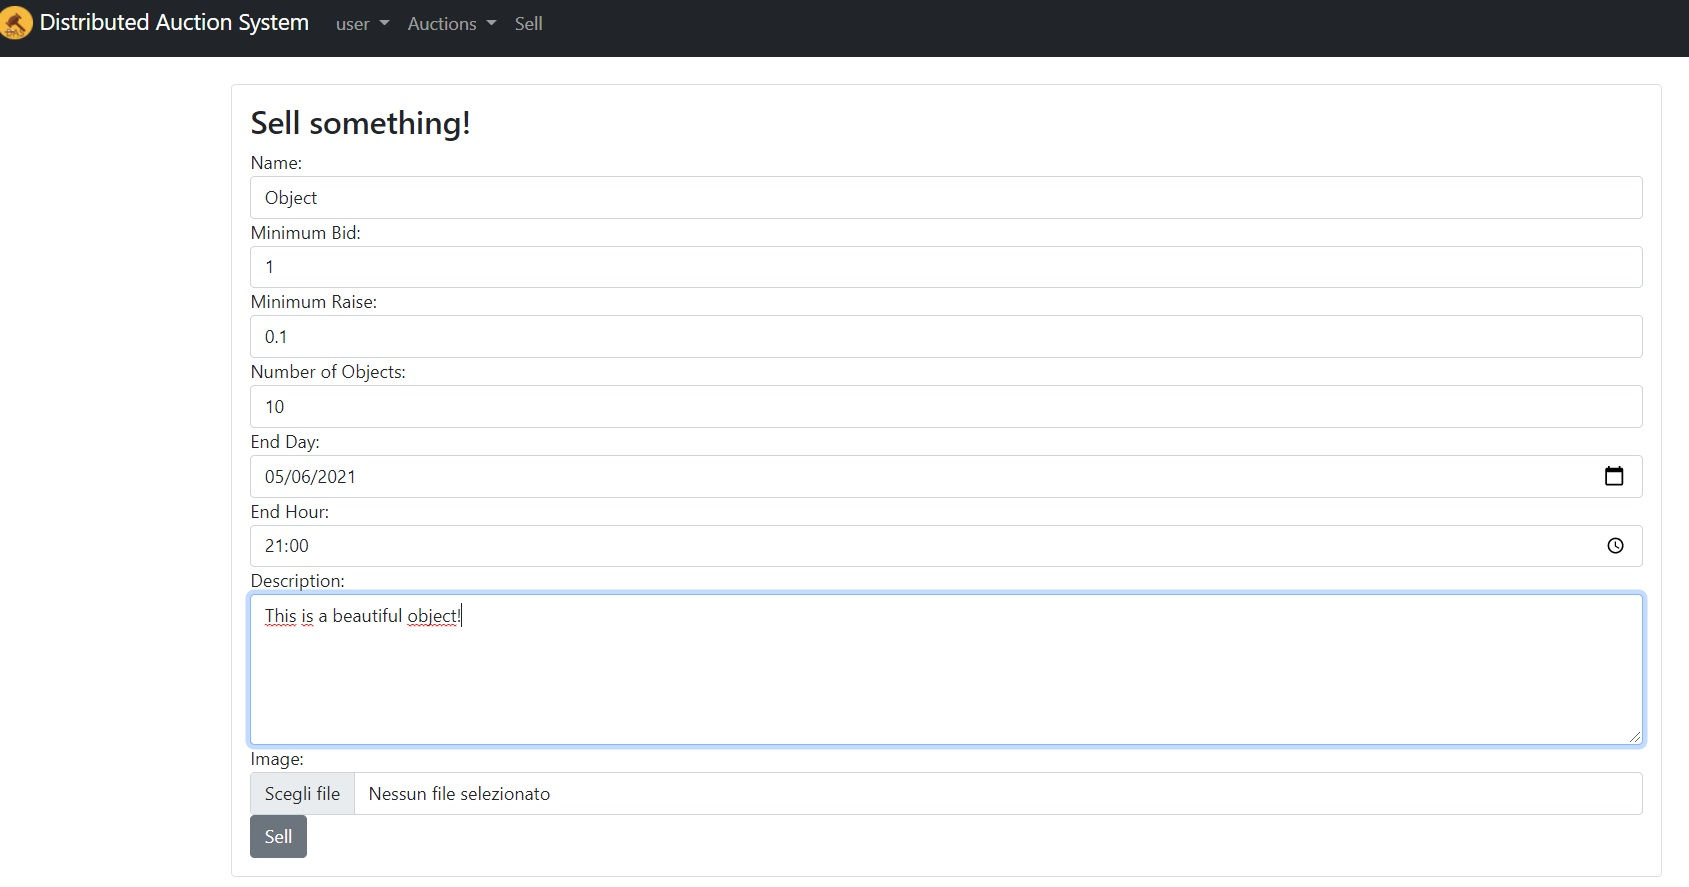
\includegraphics[width=\textwidth]{img/sell.jpg}
	\caption{Creation of a new auction}\label{fig:create-auction}
\end{figure}
